\chapter{Gale Polytopes}
\label{chap:GalePolytopes}
Recall Gale's evenness condition, which exactly describes the facets of the cyclic polytope \(\cyc nd\) of dimension \(d\) with \(n\) vertices.
\begin{GEC}
    A subset \(S\sbset \brac n\) with \(\card S=d\) forms a facet of \(\cyc nd\) if and only if
        \[
            \card{\setb{k}{k\in S\text{ and }i<k<j}}\text{ is even for all } i<j,\, \seta{i,j}\cap S=\mt
        \]
\end{GEC}

It is reasonable to ask if a noncyclic polytope satisfies a weakened form of Gale's evenness condition, namely:
\begin{Definition}
    A \(d\)-polytope \(P\) with vertex set \(\vrt(P)=\seta{\ve v_1, \ve v_2\dc \ve v_n}\) is called a \dfn{Gale} polytope if there is an ordering of \(\vrt(P)\) such that each facet satisfies the following property:

    If \(S\sbset\brac n\) and \(F\) is a facet of \(P\) with \(\vrt(F)=\setb{\ve v_{s}}{s\in S}\), then
        \[
            \card{\setb{k}{k\in S\text{ and }i<k<j}}\text{ is even for all } i<j,\, \seta{i,j}\cap S=\mt.
        \]
\end{Definition}

An equivalent characterization is as follows:

Let \(P\) be a polytope,  \(\ve v_1, \ve v_2\dc\ve v_n\) be an ordering of \(\vrt(P)\) and \(S=\seta{\ve v_{i_1}, \ve v_{i_2}\dc \ve v_{i_k}}\sbset\vrt(P)\) be such that \(i_1<i_2<\dotsb<i_k\).  Then a \dfn{block} of \(S\) is a subset \(C\) of \(S\) such that if \(t=\min\setb{i_j}{\ve v_{i_j}\in C}\), then there is some \(r\in \N\) such that \(C=\seta{\ve v_t, \ve v_{t+1}\dc \ve v_{t+r-1}}\) and \(\ve v_{t+r}\notin S\).  In this case, the \dfn{length} of a block is \(\card{C}=r\).

\begin{Definition}
    A polytope \(P\) is \dfn{Gale} if there is an ordering of \(\vrt(P)\) such that if \(F\) is a facet of \(P\), then for each block \(G\) of \(\vrt F\)  one of the following holds:
        \begin{enumerate}
            \item   the length of \(G\) is even; or
            \item   \(\ve v_1\in G\); or
            \item   \(\ve v_n\in G\).
        \end{enumerate}
    Such an ordering of the vertices is called a \emph{Gale ordering}.  A block which contains \(\ve v_1\) is called an \dfn{initial block}.  A block which contains \(\ve v_n\) is called a \dfn{terminal block}.  A block which is neither initial, nor terminal is called \dfn{internal}.
\end{Definition}

In terms of blocks, a polytope is Gale if and only if there is an ordering of the vertices such that in each facet the only blocks of odd length are either initial, or terminal.  Note that a facet need not have either an initial block, or a terminal block.

An immediate consequence of either definition is:  If \(P\) is a Gale polytope with \(n\) vertices, and \(\ve v_1, \ve v_2\dc \ve v_n\) is a Gale ordering of \(\vrt(P)\), then so is \(\ve v_n, \ve v_{n-1}\dc \ve v_1\).  Note that all cyclic polytopes are Gale, and therefore all polytopes of dimension less than or equal to \(2\) are Gale.

\begin{Theorem}
    If \(P\) is a Gale polytope, then so is \(\pyr(P)\), a pyramid over \(P\).
\end{Theorem}
\begin{proof}
    Let \(\ve v_1, \ve v_2\dc\ve v_n\) be a Gale ordering of \(\vrt(P)\) and \(\ve w_1, \ve w_2\dc\ve w_{n+1}\) be the ordering of \(\vrt(\pyr(P))\) with \(\ve w_i\) corresponding to \(\ve v_i\) for \(i\in\brac n\), and with \(\ve w_{n+1}\) as the apex of the pyramid.

    Let \(F\) be a face of \(\pyr(P)\).  Then either \(\vrt(F)=\seta{\ve w_1,\ve w_2\dc\ve w_n}\), or \(\ve w_{n+1}\in \vrt(F)\).  In the first case, \(F\) contains only an initial block.

    In the second case, write \(\vrt(F)=\seta{\ve w_{i_1},\ve w_{i_2}\dc\ve w_{i_k},\ve w_{n+1}}\) with \(i_1<i_2<\dotsb<i_k<n+1\).  Then either \(i_k=n\), or \(i_k<n\).  If \(i_k=n\), then each block \(C\) of \(\seta{\ve w_{i_1},\ve w_{i_2}\dc\ve w_{i_k}}\) satisfies at least one of the following: \(C\) is internal of even length; \(C\) is initial; or \(\ve w_n\in C\).  Thus, after adding in \(\ve w_{n+1}\), each block \(C'\) satisfies one of the following respectively: \(C'\) is internal of even length; \(C'\) is initial; or \(C'\) is terminal.  In the case that\ \(i_k<n\), each block of \(\seta{\ve w_{i_1},\ve w_{i_2}\dc\ve w_{i_k}}\) is either initial, or is of even length.  Ergo, when \(\ve w_{n+1}\) is added the only change is that a terminal block of length \(1\) is added.
\end{proof}

\begin{Theorem}
    Suppose \(P\) is a Gale polytope, and let \(X\) be a collection of pairwise disjoint facets that each have an odd number of vertices.  Then \(\card X\le 2\) .
\end{Theorem}
\begin{proof}
    Let \(P\) be a Gale polytope, and \(F\) be a facet of \(P\) which has an odd number of vertices.

    Consider the blocks of \(F\). since \(F\) has an odd number of vertices, it must have either an initial or terminal block.  If this were not the case, then there would be an internal block with an odd number of vertices.
\end{proof}

\begin{Example}
    The above theorem shows that both the regular dodecahedron and regular icosahedron are not Gale polytopes.  The shaded facets in Figure \ref{Fig:RegDodeca} are all disjoint with an odd number of vertices, and there are more than two in each polytope.
    \begin{figure}[ht]
        \centering
            \includegraphics[width=.6\textwidth, page=24]{pictures.pdf}
        \caption{The regular dodecahedron and icosahedron are not Gale polytopes.\label{Fig:RegDodeca}}
    \end{figure}
\end{Example}

If \(P\) is a \(3\)-polytope with five or fewer vertices then it is combinatorially equivalent to one of \(\simp3\), \(\pyr(\cyc24)\), or \(\cyc35\) each of which is Gale.  However, there is a \(3\)-polytope with six vertices which is not Gale.  In order to demonstrate this, we will use Theorem \ref{Thm:SimpGale} which is a consequence of Lemma \ref{Thm:KleeMinty}.  For a proof, see \cite{KleeMinty}.
\begin{Lemma}[Klee, Minty 1972]\label{Thm:KleeMinty}
    Let \(X\) and \(Y\) be polytopes having the same number \(m\) of vertices, the vertices of \(X\) being \(\ve x_1,\ve x_2\dc\ve x_m\) and those of \(Y\) being \(\ve y_1,\ve y_2\dc\ve y_m\).  Suppose that for each index set \(I\sbset\brac m\),
        \[
            \conv\setb{\ve x_i}{i\in I}\text{ is a facet of }X
                \text{ implies }
                    \conv\setb{\ve y_i}{i\in I}\text{ is a facet of }Y.
        \]
    Then the reverse implications hold, whence \(X\) and \(Y\) are combinatorially equivalent.
\end{Lemma}

The following theorem is found in \cite{BayerBisz}.

\begin{Theorem}\label{Thm:SimpGale}
    If \(P\) is a simplicial Gale polytope, then \(P\) is a cyclic polytope.
\end{Theorem}
\begin{proof}
    First, recall that if \(\vrt(\cyc nd)=\seta{\ve v_1,\ve v_2\dc\ve v_n}\), then the set facets of \(\cyc{n}d\) is
        \[
            X=\setb{\conv\seta{\ve v_{i_1},\ve v_{i_2}\dc\ve v_{i_{d+1}}}}{\seta{\ve v_{i_1},\ve v_{i_2}\dc\ve v_{i_{d+1}}}\text{ satisfies Gale's evenness condition}}.
        \]

    Let \(P\) be a simplicial Gale polytope of dimension \(d\) with \(\card{\vrt{P}}=n\).  Then there is some ordering \(\ve w_1, \ve w_2\dc\ve w_n\) of \(\vrt P\) such that if \(\conv\seta{\ve w_1,\ve w_2\dc\ve w_{i_{d}}}\) is a facet of \(P\), then the set \(\conv\seta{\ve v_{i_1},\ve v_{i_2}\dc\ve v_{i_{d}}}\) is a facet of \(\cyc nd\) since the set of facets of \(\cyc nd\) is \(X\).

    Thus \(P\) and \(\cyc nd\) satisfy the hypothesis of Lemma \ref{Thm:KleeMinty}.  Hence \(P\) is combinatorially equivalent to \(\cyc nd\).
\end{proof}
\begin{comment}
\begin{proof}
    Thus, the map \(\ve w_i\mapsto\ve v_i\) induces a map \(\varphi\colon\fl P\rightarrow\fl{\cyc nd}\) from the face lattice of \(P\) to that of \(\cyc nd\) which is an injection.

    Suppose \(F=\conv\seta{\ve v_{i_1},\ve v_{i_2}\dc\ve v_{i_{d+1}}}\) is a facet of \(\cyc nd\) such that \(\varphi\nv F\)
    %=\conv\seta{\ve w_{i_1},\ve w_{i_2}\dc\ve w_{i_{d+1}}}
    is not a facet of \(P\).  Let \(F'\) be any facet of \(P\).  Then there is a sequence \(F=F_1,F_2\dc F_r=\varphi F'\) of facets of \(\cyc nd\) such that \(\card{\vrt(F_i)\cap\vrt(F_{i+1})}=d-1\) for each \(i\in\brac{r-1}\).  Thus, there is some \(t\) such that \(\varphi\nv F_1,\varphi\nv F_2\dc\varphi\nv F_t\) are not facets of \(P\), but \(\varphi\nv F_{t+1}\) is.

    Let \(R=F_t\cap F_{t+1}\).  Then \(R\in\fl{\cyc nd}\) since \(\fl{\cyc nd}\) is a lattice, and \(\varphi\nv R\in\fl{P}\) since \(P\) is simplicial and \(\varphi\nv R\sbset\varphi\nv F_t\in\fl P\).

    Since \(P\) is a polytope, there is some \(K\in\fl P\) such that \(\varphi\nv R\varsubsetneq K\varsubsetneq P\) with \(K\ne \varphi\nv F_{t+1}\)  \cite[page 57]{ZieglerBook}.  Similarly, if \(L\in\fl{\cyc nd}\) such that \(R\varsubsetneq L\varsubsetneq \cyc nd\), then either \(L=F_t\), or \(L=F_{t+1}\).  Since \(\varphi\) is an injection, it must be the case that \(\varphi K= F_t\).  Thus \(\varphi\) is an isomorphism, and \(P\) is cyclic.
\end{proof}
\end{comment}

Thus, for example, \(\xp3\) is not a Gale polytope since each vertex of \(\xp3\) lies on four edges, whereas \(\cyc36\) has two vertices which each lie on only three edges.

Since simplices are cyclic polytopes, and cyclic polytopes are simplicial, each facet of a cyclic polytope satisfies Gale's evenness condition.  However, this need not happen for a general Gale polytope.  The following is an example of a Gale polytope with a facet which is not Gale.

\begin{Example}
    Consider the \(5\)-dimensional cyclic polytope with vertices \(\ve x_1,\ve x_2,\ve x_3,\ve x_4,\ve x_5,\ve x_6,\ve x_7\).  Let \(P\) be a vertex figure of \(\cyc75\) at \(\ve x_4\).  Then \(P\) is a \(4\)-dimensional simplicial polytope with \(6\) vertices \(\ve z_1,\ve z_2,\ve z_3,\ve z_5,\ve z_6,\ve z_7\) (where \(\ve z_i\) corresponds to the edge \(\ve x_4\ve x_i\)).

    The facets of \(P\) are the convex hulls of the following sets:
        \begin{align*}
            \seta{\ve z_1, \ve z_2, \ve z_3, \ve z_5}&&
            \seta{\ve z_1, \ve z_2, \ve z_3, \ve z_7}&&
            \seta{\ve z_1, \ve z_2, \ve z_5, \ve z_7}&&
            \seta{\ve z_1, \ve z_3, \ve z_5, \ve z_6}&\\
            \seta{\ve z_1, \ve z_3, \ve z_6, \ve z_7}&&
            \seta{\ve z_1, \ve z_5, \ve z_6, \ve z_7}&&
            \seta{\ve z_2, \ve z_3, \ve z_5, \ve z_7}&&
            \seta{\ve z_3, \ve z_5, \ve z_6, \ve z_7}&.
        \end{align*}

    Let \(Q\) be a pyramid over \(P\) with apex \(\ve a\).  Then \(Q\) is a Gale polytope with Gale ordering
        \[
            \ve z_1,\ve z_2,\ve z_3,\ve a,\ve z_5,\ve z_6,\ve z_7.
        \]
    However, \(P\) (which is the base of the pyramid \(Q\), and therefore also a facet of \(Q\)) is not Gale since it is a simplicial \(4\)-polytope whose graph is not complete (it is missing the edge \(\conv\seta{\ve z_2,\ve z_6}\)) and therefore \(P\) is not cyclic.

    Notice that this construction generalizes to give infinitely many polytopes with this property.  Consider the cyclic polytope \(\cyc{2n+1}d\) (of dimension at least \(4\)) with an odd number of vertices.  Let \(P\) be a vertex figure of \(\cyc{2n+1}d\) at the vertex \(n+1\), and \(Q\) be a pyramid over \(Q\).
\end{Example}

\begin{Theorem}\label{Thm:GaleProduct}
    If \(P\) is a Gale \(d\)-polytope, and \(Q\) is a Gale \(d'\)-polytope, then \(P\times Q\) is a Gale \((d+d')\)-polytope.
\end{Theorem}

\begin{proof}
Suppose \(\ve v_1,\ve v_2\dc \ve v_n\) is a Gale ordering of \(\vrt(P)\), and \(\ve w_0,\ve w_1\dc \ve w_m\) is a Gale ordering of \(\vrt Q\).  Then define an ordering of \(\vrt(P\times Q)\) as follows:

Let \((V_1,\ve w_i)\) and \((V_{-1},\ve w_i)\) respectively be the sequences:
    \begin{align*}
        &(\ve v_1,\ve w_i),(\ve v_2,\ve w_i)\dc(\ve v_n,\ve w_i)\\
        &(\ve v_n,\ve w_i),(\ve v_{n-1},\ve w_i)\dc(\ve v_1,\ve w_i).
    \end{align*}
Define similarly, \((B_1,\ve w_i)\) and \((B_{-1},\ve w_i)\) for \(B\) a set of vertices of \(P\).

Claim: \((V_1,\ve w_0),(V_{-1},\ve w_1)\dc(V_{(-1)^m},\ve w_m)\) is a Gale ordering of \(P\times Q\).

First, consider the facets of \(P\times Q\) of the form \(P\times G\) where \(G\) is a facet of \(Q\).  The vertex \(\ve w_j\) is a vertex of \(G\) if and only if \((\ve v_i, \ve w_j)\) is a vertex of the facet \(P\times G\) for each \(\ve v_i\in\vrt(P)\).  In particular, the sequence \((V_{(-1)^j},\ve w_j)\) is part of a block of \(P\times G\).

If \(n\) is even, then each of these parts is of even length, and hence every block of \(P\times G\) is even.  If \(n\) is odd, then consider the blocks of \(G\).  If \(G\) has an initial block \(\ve w_0,\ve w_1\dc \ve w_t\), then \(P\times G\) has initial block \((V_1,\ve w_0),(V_{-1},\ve w_1)\dc (V_{(-1)^t},\ve w_t)\) (since \((\ve v_1,\ve w_{t+1})\) is not a vertex of \(P\times G\)).  A similar statement applies for terminal blocks.

Suppose that \(G\) has an internal block \(\ve v_k,\ve v_{k+1}\dc\ve v_{k+s-1}\).  Since this is an internal block, \(s\) must be even.  Thus the sequence \((V_{(-1)^k},\ve w_k),(V_{(-1)^{k+1}},\ve w_{k+1})\dc(V_{(-1)^{k+s-1}},\ve w_{k+s-1})\) is an internal block of \(P\times G\) of length \(\card{\vrt(P)}\cdot s\) (this is an even number).  This follows since each element of the above sequence is a vertex of \(P\times G\), and none of the vertices
    \[
        (\ve v_1,\ve w_{k-1}), (\ve v_n,\ve w_{k-1}), (\ve v_n,\ve w_{k+s}), (\ve v_1,\ve w_{k+s})
    \]
is a vertex of \(P\times G\).

Now, consider the facets of \(P\times Q\) of the form \(F\times Q\) with \(F\) a facet of \(P\).  In this case, similar to above, \(\ve v_i\in F\) if and only if \((\ve v_i,\ve w_j)\in F\times Q\) for each \(j\in\brac m\cup\seta0\).  The sequence \(B=\ve v_i,\ve v_{i+1}\dc\ve v_{i+k-1}\) is part of a block of \(F\) if and only if
    \begin{align*}
        \begin{cases}
            (B_1,\ve w_j)=
                (\ve v_i,\ve w_j),(\ve v_{i+1},w_j)\dc (\ve v_{i+k-1},\ve w_j)
                    &   ,j\text{ even}\\
            (B_{-1},\ve w_j)=
                (\ve v_{i+k-1},\ve w_j),(\ve v_{i+k-2},w_j)\dc(\ve v_i,\ve w_j)
                    &   ,j\text{ odd}\\
        \end{cases}
    \end{align*}
is part of a block of \(F\times Q\).  If \(B\) is an internal block of \(F\), then the above are internal blocks of \(F\times Q\).

Suppose that \(B\) is an initial block of \(F\) (in particular, \(i=1\), and \(B\) has length \(k\)).  Then:
    \begin{itemize}
        \item   \((B_1,\ve w_1)\) is an initial block of \(F\times Q\);
        \item   if \(m\) is odd, then \((B_{-1},\ve w_m)\) is a terminal block of \(F\times Q\);
        \item   if \(m\) is even, then \((B_{-1},\ve w_{m-1}),(B_1,\ve w_m)\) is an internal block of length \(2k\).
    \end{itemize}
Further, \((B_{-1},\ve w_{2\ell-1}),(B_1,\ve w_{2\ell})\) is an internal block of length \(2k\) for \(\ell\in\brac{\floor{m/2}}\).

The case that \(B\) is a terminal block is handled similarly.
\end{proof} 